\documentclass[pdftex,fleqn,a4paper]{article}

  \let\oldAuthor\author
  \renewcommand{\author}[1]{\newcommand{\theAuthor}{#1}\oldAuthor{#1}}
  \let\oldTitle\title
  \renewcommand{\title}[1]{\newcommand{\theTitle}{#1}\oldTitle{#1}}
  \newcommand{\subtitle}[1]{\newcommand{\theSubtitle}{#1}}
  \let\oldDate\date
  \renewcommand{\date}[1]{\newcommand{\theDate}{#1}\oldDate{#1}}

  \usepackage{vubtitlepage}
 \faculty{Faculteit Ingenieurswetenschappen}

  \author{\href{mailto:Egon.Geerardyn@vub.ac.be}{Egon Geerardyn}}
  \title{Formules Mechanica}
  \newcommand{\revisie}{revisie 1.7}
  \date{\revisie\ (\today)}




  %\usepackage{graphicx}

  \usepackage{fancyhdr}
  \usepackage[dutch]{babel}
  \usepackage[utf8]{inputenc}
  \usepackage[T1]{fontenc}
  \usepackage[pdftex]{hyperref}
  \usepackage{graphicx}
  \usepackage{wrapfig}
  \usepackage{flow}
  %%%%

  \addtolength{\textheight}{2cm}
  \addtolength{\textwidth}{3cm}
  \addtolength{\hoffset}{-1.5cm}
  \renewcommand{\rmdefault}{cmss}
  \renewcommand{\sfdefault}{cmr}


    \renewcommand{\vec}[1]{\overline{#1}} %small notations (may be commented out for traditional arrow notation)
    \input{../commands/commands.inc.tex}

 %lay-out
  \hypersetup{colorlinks,%
            citecolor=black,%
            filecolor=black,%
            linkcolor=black,%
            urlcolor=black,%
            pdfauthor={Egon Geerardyn},%
            pdftitle={Formules Mechanica},%
            plainpages=false}
  \pdfpagewidth=\paperwidth
  \pdfpageheight=\paperheight
 %margins
\begin{document}
 \maketitlepage
%  \titlepage
%  \thispagestyle{empty}%
%  \null
%  \vfill
%  \begin{center}\leavevmode
%    \normalfont
%    %{\Large\raggedleft schooljaren 2004 -- 2005 -- 2006\par}%
%    {\Large\raggedleft Ingenieurswetenschappen\par}%
%    \hrulefill\par
%    {\Huge\raggedright Formularium Mechanica \large \revisie\   \footnotesize (\today)\par }%
%  \end{center}%
%  \vfill
%  \scriptsize{auteur: \textsc{E. Geerardyn}\par
%  \scriptsize{bron: \textsc{prof. D. Lefeber}, \textit{Mechanica: Deel I}, Dienst Uitgaven VUB 2006.}\par
%  \scriptsize{bron: \textsc{prof. D. Lefeber}, \textit{Mechanica: Deel II}, Dienst Uitgaven VUB 2006.}
%  \normalsize
%
%  \null
\setlength{\voffset}{-2cm}
  \newpage

  \pagestyle{fancy}
  \rhead{pagina \thepage}
  \chead{\footnotesize \revisie}
  \lhead{\textbf{Formules Mechanica}}
  \cfoot{}
  \section*{Voorwoord}
\label{sec:Voorwoord}
  Deze uitgave is geen officiële uitgave van de Vrije Universiteit Brussel, slechts een formularium gemaakt door een student.
  Mogelijk staan er hier of daar nog fouten in, indien u er tegenkomt,
  stuur gerust een mailtje naar \hreftt{mailto:egon.geerardyn@vub.ac.be}{egon.geerardyn@vub.ac.be}.\par

  \begin{quote}
    Copyright \copyright{}  Egon Geerardyn.\par
    Permission is granted to copy, distribute and/or modify this document
    under the terms of the GNU Free Documentation License, Version 1.2
    or any later version published by the Free Software Foundation;
    with no Invariant Sections, no Front-Cover Texts, and no Back-Cover Texts.
    A copy of the license is included in the section entitled ``GNU
    Free Documentation License'' in the source code and available on:
    \linktt{http://www.gnu.org/copyleft/fdl.html}.
  \end{quote}
  \noindent
  De \LaTeX -broncode is vrij beschikbaar onder GNU Free Document License. \par


  Mogelijk is er reeds een nieuwe versie beschikbaar op\par
  \hreftt{http://students.vub.ac.be/~egeerard/projects.html}{http://students.vub.ac.be/\tildefix egeerard/projects.html}
\section*{Referenties}
\begin{enumerate}
	\item \textsc{D. Lefeber}, \textit{Mechanica: Deel I}, Dienst Uitgaven VUB 2006.
	\item \textsc{D. Lefeber}, \textit{Mechanica: Deel II}, Dienst Uitgaven VUB 2006.
        \item \textsc{D. Lefeber}, \textit{Mechanica met ontwerpproject}, Polytechnische Kring 2007.
        \item \textsc{D. Van Hemelrijck}, \textit{Mechanica van materialen, mechanismen en vloeistoffen}, Pointcarré 2008.
	\item \textsc{D. Vandepitte}, \linktt{http://www.berekeningvanconstructies.be}, 2006.
\end{enumerate}



   \newpage
   \tableofcontents
   \newpage

   \input{vectoren.inc.tex}
   \newpage
\twocolumn
\section{Coördinatentransformaties}
\label{sec:Coordinatentransformaties}

\subsection{Poolcoördinaten}
\label{sec:PoolCoords}
Plaats
\[
  \left\{
    \begin{array}{rcl}
      r_x & = & r \cos \theta\\
      r_y & = & r \sin \theta
    \end{array}
  \right.
\]
Snelheid
\[
  \left\{
    \begin{array}{rcl}
      v_{r}      & = & \dt{r}\\
      v_{\theta} & = & r \dt{\theta}
    \end{array}
  \right.
\]
Versnelling
\[
  \left\{
    \begin{array}{rcl}
      a_{r}      & = & \dtt{r} - r\dt{\theta}\\
      a_{\theta} & = & r\dtt{\theta} + 2\dt{r}\dt{\theta}
    \end{array}
  \right.
\]

\subsection{Cilindercoördinaten}
\label{sec:CilinderCoords}
Plaats
\[
  \left\{
    \begin{array}{rcl}
      r_x & = & r \cos \theta\\
      r_y & = & r \sin \theta\\
      r_z & = & z
    \end{array}
  \right.
\]
Snelheid
\[
  \left\{
    \begin{array}{rcl}
      v_{r}      & = & \dt{r}\\
      v_{\theta} & = & r \dt{\theta}\\
      v_z        & = & \dt{z}
    \end{array}
  \right.
\]
Versnelling
\[
  \left\{
    \begin{array}{rcl}
      a_{r}      & = & \dtt{r} - r\dt{\theta}\\
      a_{\theta} & = & r\dtt{\theta} + 2\dt{r}\dt{\theta}\\
      a_{z}      & = & \dtt{z}
    \end{array}
  \right.
\]

\subsection{Bolcoördinaten}
\label{sec:BolCoords}
Plaats
\[
  \left\{
    \begin{array}{rcl}
      r_x & = & r \sin \theta \cos \varphi\\
      r_y & = & r \sin \theta \sin \varphi\\
      r_z & = & r \cos \theta
    \end{array}
  \right.
\]
Snelheid
\[
  \left\{
    \begin{array}{rcl}
      v_{r}       & = & \dt{r}\\
      v_{\theta}  & = & r \dt{\theta}\\
      v_{\varphi} & = & r \dt{\varphi} \sin \theta
    \end{array}
  \right.
\]
Versnelling
\[
  \left\{
    \begin{array}{rcl}
      a_{r}      & = & \dtt{r} - r \dt{\varphi}^2 \sin^2 \theta - r \dt{\theta}\\
      a_{\theta} & = & r \dtt{\theta} + 2 \dt{r}\dt{\theta} - r \dt{\varphi}^2 \sin \theta \cos \theta\\
      a_{z}      & = & r \dtt{\varphi} \sin \theta + 2 \dt{r}\dt{\varphi} \sin \theta + 2r \theta \dt{\varphi}\cos \theta 
    \end{array}
  \right.
\]

\onecolumn

   \newpage
\onecolumn
\section{Kinematica van een Punt}
\label{sec:KinematicaPunt}


\subsection{Baan van een Punt}
\label{sec:BaanPunt}
\[
  \vec{r} = \vec{r}\left( t \right) =
  \left\{
        \begin{array}[h]{lcr}
	       x & = & x\left( t \right)\\
	       y & = & y\left( t \right)\\
	       y & = & y\left( t \right)\\
        \end{array}
  \right.
\]

\paragraph{Elementaire Booglengte}
\label{sec:ElementaireBooglengte}
\[
  \d{s} = \sqrt{\d{x}^2 + \d{y}^2 + \d{z}^2}
\]

\paragraph{Normaalvlak} \textbf{N} in $P$
\label{sec:Normaalvlak}
\[
  \vect{XP} \cdot \vec{1}_t = 0
\]
\[
  \ds{x}_P \left(x-x_P\right) + \ds{y}_P \left(y-y_P\right) + \ds{z}_P \left(z-z_P\right) = 0
\]
Vlak door $P$ met als normaalvector de raakvector aan de baan $\vec{1}_t$

\paragraph{Osculatievlak} \textbf{O} in $P$
\label{sec:Osculatievlak}
\[
  \left( \vec{v}_P \times \vec{a}_P \right) \cdot \vect{PX} = 0
  \Leftrightarrow
  \left( \dt{\vec{r}} \times \dtt{\vec{r}} \right) \cdot \vect{PX} = 0
\]
\[
  \left|
    \begin{array}{cccc}
     x       & y       & z       & 1 \\
     x_P     & y_P     & z_P     & 1 \\
     \dt{x}  & \dt{y}  & \dt{z}  & 0 \\
     \dtt{x} & \dtt{y} & \dtt{z} & 0 \\
    \end{array}
  \right|
  =
  \left|
    \begin{array}{ccc}
     x-x_P   & y-y_P   & z - z_P \\
     \dt{x}  & \dt{y}  & \dt{z}  \\
     \dtt{x} & \dtt{y} & \dtt{z} \\
    \end{array}
  \right|
  = 0
\]
Vlak door $P$ met als normaalvector de binormale $\dt{\vec{r}} \times \dtt{\vec{r}} $.

\paragraph{Raaklijn} \textbf{R} in $P$
\label{sec:Raakvlak}
\[
  \vec{OQ} = \vec{P} + k\vec{1}_t = \vec{P} + k\frac{\d{\vec{r}}}{\d{s}}
\]
Drager van de snelheidsvector in $P$, loodrecht op de plaatsvector.

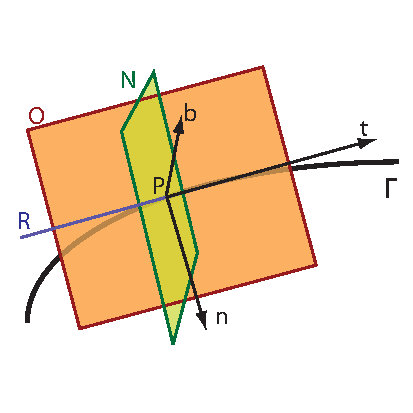
\includegraphics{Figuren/Vlakken.pdf}


\subsection{Snelheid van een Punt}
\label{sec:SnelheidPunt}
\[
  \vec{v} = \dt{\vec{r}}
          = \frac{\d{\vec{r}}}{\d{t}}
          = \frac{\d{x}}{\d{t}} \vec{1}_x + \frac{\d{y}}{\d{t}} \vec{1}_y + \frac{\d{z}}{\d{t}} \vec{1}_z
          = \dt{x} \vec{1}_x + \dt{y} \vec{1}_y + \dt{z} \vec{1}_z
\]
\[
  v       = \norm{\vec{v}}
          = \dt{s}
          = \frac{\d{s}}{\d{t}}
\]
\[
  \vec{v} = \norm{\vec{v}} \vec{1}_t
          = v \vec{1}_t
\]
\subsection{Versnelling van een Punt}
\label{sec:VersnellingPunt}
\[
  \vec{a} = \dt{\vec{v}}
          = \dtt{\vec{r}}
          = \frac{\d{^2 \vec{r}}}{\d{t^2}}
          = \frac{\d^2{x}}{\d{t^2}} \vec{1}_x + \frac{\d^2{y}}{\d{t^2}} \vec{1}_y + \frac{\d^2{z}}{\d{t^2}} \vec{1}_z
          = \dtt{x} \vec{1}_x + \dtt{y} \vec{1}_y + \dtt{z} \vec{1}_z
\]
\[
  \vec{a} = \dt{v} \vec{1}_t + \frac{v^2}{R} \vec{1}_n
          = \frac{\d{v}}{\d{t}} \vec{1}_t + \frac{v^2}{R} \vec{1}_n
          \qquad \qquad \mbox{ontbinding van Huygens}
\]
\[
  a^2    = \norm{\vec{a}}^2
         = \left( \frac{\d{v}}{\d{t}} \right)^2 + \frac{v^4}{R^2}
         = \dt{v}^2 + \frac{v^4}{R^2}
\]

\subsection{Drievlakshoek van Frenet}
\label{sec:DrievlakshoekFrenet}
\[
  \left( \vec{1}_t , \vec{1}_n , \vec{1}_b\right)
\]
\[
  \vec{1}_t \times \vec{1}_n = \vec{1}_b
\]
\[
  \vec{1}_b = \frac{\dt{\vec{r}} \times \dtt{\vec{r}}}{\norm{\dt{\vec{r}} \times \dtt{\vec{r}}}}
\]
\[
  \vec{1}_t = \frac{\dt{\vec{r}}}{\norm{\dt{\vec{r}}}}
            = \frac{\vec{v}}{\norm{\vec{v}}}
            = \frac{\dt{\vec{r}}}{\dt{s}}
            = \frac{\d{\vec{r}}}{\d{s}}
            = \ds{\vec{r}}
\]
\[
  \vec{1}_n = \vec{1}_b \times \vec{1}_t
\]

\subsection{Formules van Frenet}
\label{sec:FormulesFrenet}
\[
  \frac{\d{\vec{1}_t}}{\d{s}} = \frac{1}{R}\vec{1}_n
\]
\[
  \frac{\d{\vec{1}_b}}{\d{s}} = \frac{1}{T}\vec{1}_n
\]
\[
  \frac{\d{\vec{1}_n}}{\d{s}} = - \frac{1}{R} \vec{1}_t - \frac{1}{T} \vec{1}_b
\]

\subsection{Kromtecirkel en Kromtestraal}
\label{sec:KromtecirkelEnKromtestraal}
\[
 \rho = R = \pm \frac{\d{s}}{\d{\alpha}} > 0
\]

\paragraph{Kromtestraal met baan in parametervorm}
\label{sec:KromtestraalParametervorm}
$\Gamma : x\left(t\right), y\left(t\right)$
\[
  \rho = \pm \frac{\left(\dt{x}^2 + \dt{y}^2\right)^{3/2}}{\dt{x}\dtt{y} + \dt{y}\dtt{x}}
\]

\paragraph{Kromtestraal met baan in natuurlijke parametervorm}
\label{sec:KromtestraalNatuurlijkeParametervorm}
$\Gamma : x\left(s\right), y\left(s\right)$
\[
  \rho = \pm \frac{1}{\ds{x}\dss{y} + \ds{y}\dss{x}}
\]

\paragraph{Kromtestraal met baan als functievoorschrift}
\label{sec:KromtestraalFunctievorm}
$\Gamma : y = y\left( x \right)$
\[
  \rho = \pm \frac{\left(1 +\dx{y}^2\right)^{3/2}}{\dxx{y}} \qquad \qquad \mbox{met } \dx{} = \frac{\d{}}{\d{x}}
\]

\paragraph{Kromtestraal in 3 dimensies}
\label{sec:Kromtestraal3D}
$\Gamma : x\left(t\right), y\left(t\right), z\left(t\right)$
\[
  R = \frac{1}{\sqrt{\dss{x}^2 + \dss{y}^2 + \dss{z}^2}}
\]

\subsection{Perksnelheid en -versnelling}
\label{sec:Perksnelheid}
\[
  \vec{v}_{perk} = \frac{\d{\vec{S}}}{\d{t}} = \frac{1}{2} \vect{OP} \times \vec{v} = \frac{1}{2} \vec{M}_O (\vec{v})
\]
\[
  \vec{a}_{perk} = \frac{\d^2{\vec{S}}}{\d{t}^2} = \frac{1}{2} \vect{OP} \times \vec{a} = \frac{1}{2} \vec{M}_O (\vec{a})
\]

\subsection{Relatieve beweging}
Een index $_O$ slaat op de oorsprong van het relatief assenstelsel.
Een index $_R$ slaat op de coördinaten in het relatief assenselsel.
Let op de gebruikte assenstelsel bij het onbinden in componenten!
\[
  \vec{r} = \vec{r}_O + \vec{r}_R
\]
\[
  \vec{v} = \vec{v}_R + \vec{v}_s
\]
\[
  \vec{a} = \vec{a}_R + \vec{a}_s + \vec{a}_c
\]
Hierin zijn:
\[
  \vec{v}_s = \vec{v}_O + \vec{\omega} \times \vec{r}_R
\]
\[
  \vec{a}_s = \vec{a}_O + \dt{\vec{\omega}} \times \vec{r}_R + \vec{\omega} \times \left( \vec{\omega} \times \vec{r}_R \right)
\]
\[
  \vec{a}_c = 2 \vec{\omega} \times \vec{v}_R
\]




   \newpage
\section{Statica}
\label{sec:Statica}

\subsection{Stelsels van glijdende vectoren}
\label{sec:StelselsVanGlijdendeVectoren}
  \paragraph{Elementaire bewerkingen}
  \label{sec:ElemBewerkingGelijkwStelsels}
    \begin{itemize}
	    \item Twee tegengestelde vectoren op eenzelfde drager toevoegen (en omgekeerd)
	    \item Twee vectoren met samenlopende (snijdende) dragers vervangen door hun resultante (en omgekeerd)
	    \item \textbf{Varignon:} Een stelsel samenlopende vectoren is gelijkwaardig met hun algemene resultante
	    \item Een koppel is een stelsel van twee evenwijdige tegengestelde vectoren
	    \item \textbf{Poinsot:} Een stelsel kan herleid worden tot een koppel en een resultante
    \end{itemize}
  
  \subsubsection{Algemene resultante}
  \label{sec:AlgemeneResultante}
    \[
      \vec{R} = \sum_i \vec{V}_i
    \]
  \paragraph{Toepassingen en eigenschappen}
  \label{sec:eigToepAlgResultante}
    \begin{itemize}
      \item De totale resultante is gelijk in alle punten $P$ en $Q$
            \[
              \vec{R}_Q = \vec{R}_P = \vec{R}
            \]
    \end{itemize}
    
  \subsubsection{Totaal moment}
  \label{sec:TotaalMoment}
    \[
      \vec{C}_P = \sum_i \vec{M}_P \left(\vec{V}_i\right)
                = \sum_i \vect{PA_i} \times \vec{V}_i
    \]
  \paragraph{Variatie van het totaal moment}
  \label{sec:VariatietotaalMoment}
    \[
      \vec{C}_Q = \vec{C}_P + \vect{QP} \times \vec{R}_P
    \]
  \paragraph{Toepassingen en eigenschappen}
  \label{sec:eigToepVarTotaalMoment}
    \begin{itemize}
	    \item Alle punten $Q$ met eenzelfde totaal moment $\vec{C}_P = \vec{C}_Q$ als $P$, liggen op een rechte evenwijdig met de resultante
	    \item De projectie van het totaal moment in twee verschillende punten $P$ en $Q$ op de totale resultante $\vec{R}$ is constant.
	          \[
	            \frac{1}{R} \left( \vec{C}_P \cdot \vec{R} \right) = \frac{1}{R} \left( \vec{C}_Q \cdot \vec{R} \right)
	            \Leftrightarrow
	            \vec{C}_P \cdot \vec{R} = \vec{C}_Q \cdot \vec{R}
	          \]
	    \item De projectie van het totaal moment in 2 punten $P$ en $Q$ op de rechte $PQ$ is constant.
	          \[
	            \vec{C}_P \cdot \vect{PQ} = \vec{C}_Q \cdot \vect{PQ}
	          \]
	    
    \end{itemize}
  
  \subsubsection{Invarianten}
  \label{sec:Invarianten}
    \[
      \vec{R}_P = \vec{R}_Q
    \]
    \[
      \vec{C}_P \cdot \vec{R} = \vec{C}_Q \cdot \vec{R}
    \]
   
   \subsubsection{Centrale As}
   \label{sec:CentraleAs}   
   \[
     \vect{PQ} = \frac{\vec{R} \times \vec{C}_P}{\norm{\vec{R}}^2}
   \]
   \[
     \vect{OQ} = \frac{\vec{R} \times \vec{C}_0}{\norm{\vec{R}}^2} + \lambda \vec{R}
   \]
   \[
     \frac{C_{0,x} - yR_z + zR_y}{R_x} = \frac{C_{0,y} - zR_x + xR_y}{R_y} = \frac{C_{0,z} - xR_y + yR_x}{R_z}
   \]
    \paragraph{Eigenschappen}
    \begin{itemize}
      \item \[ \vec{C}_Q // \vec{R}\]
      \item \textbf{Bij een vlak stelsel vectoren (allen gelegen in 1 vlak):}
            \begin{itemize}
              \item Het stelsel is evenwaardig met 1 vector, namelijk de algemene resultante $\vec{R}$ gelegen op de centrale as
              \item Het totaal moment $\vec{C}_P$ staat loodrecht op het vlak
              \item Op de centrale as is het totaal moment $\vec{C}_Q = 0$
            \end{itemize}
      \item \textbf{Bij een stelsel evenwijdige vectoren:}
            \begin{itemize}
              \item Het stelsel is evenwaardig met 1 vector, namelijk de algemene resultante $\vec{R}$ gelegen op de centrale as
              \item Op de centrale as is het totaal moment $\vec{C}_Q = 0$
            \end{itemize}
    \end{itemize}
    
\subsection{Wrijving}
\label{sec:Wrijving}
 Bindingsreacties bij ruwe binding ontbinden in tangentiële en normale component: $\vec{R} = \vec{T} + \vec{N}$. Bij Gladde binding: $\vec{R} =  \vec{N}$
 
 \paragraph{Wrijvingscoëfficiënt en wrijvingshoek}
   \[
     f = \frac{\norm{\vec{T}}}{\norm{\vec{N}}} = \frac{T}{N} = \tan \phi
   \]
   Kinematische Wrijvingscoëfficënt ($\vec{v}_P \neq 0$)
   \[
     T = f_k N
   \]
   Statische Wrijvingscoëfficënt ($\vec{v}_P = 0$)
   \[
     T \leq f_k N
   \]
 

\subsection{Stabiliteit}
\label{sec:Stabiliteit}
Een willekeurige kleine verplaatsing $\d{\vec{r}}$ ($\vect{AA\acute{}}$) die alle bindingen respecteert kiezen en de zo onstane kracht(en) $\vec{F}$ bepalen. Bij een gladde binding hoeven de bindingsreacties niet in rekening gebracht te worden!
\[
  A = W = \vec{F} \cdot \d{\vec{r}} 
  \left\{
    \begin{array}{ll}
      < 0 \; \forall \d{\vec{r}} & \mbox{stabiel}\\
      = 0 \; \forall \d{\vec{r}} & \mbox{onverschillig}\\
      > 0 \; \mbox{voor tenminste een } \d{\vec{r}} & \mbox{instabiel}\\
    \end{array}
  \right.
\]
\paragraph{Met wrijving in rekenig gebracht:} Wrijving werkt de stabiliteit nooit tegen!
\[
  \vec{T} = -\sigma \vec{v} \qquad \mbox{$\sigma > 0$, $\vec{v}$ de glijsnelheid}
\]
\[
  \vec{R}_A \cdot \d{\vec{r}} = - \sigma v^2 \d{t} < 0
\]

\paragraph{Speciaal geval} De kracht $\vec{F}$ is de gradiënt van een potentiaal $\Phi$ of $V$:\par
Arbeid
\[
  W = A = \int \vec{F} \d{\vec{r}}
\]
\[
  \vec{F} = - \Dgrad{\Phi}
\]
\[
  A = - \int \Dgrad{\Phi} \d{\vec{r}} = - \Phi
\]
Stabiliteitsvoorwaarde
\[
  \vec{\nabla} \Phi \cdot \d{\vec{r}} = \d{\Phi} \geq 0
\]
voorbeeld:
\[
  \Phi = mgz \qquad \mbox{cfr. potentiële energie}
\] 
   
\subsection{Bepaling Massamiddelpunt}
\label{sec:BepalingMassamiddelpunt}
    \paragraph{Soortelijke Massa}
    \label{sec:SoortelijkeMassa}
      \[
        \rho\left(P\right) = \frac{\d{M}}{\d{D}} \qquad \mbox{( met $M$ massa en $D$ het domein waarvan de dichtheid bepaald wordt)}
      \]
    \paragraph{Totale Massa}
    \label{sec:totaleMassa}
      \[
        M = \int_D \rho \left( P \right) \d{D}
      \]
  \subsubsection{Discreet Massamiddelpunt}
  \label{sec:DiscreetMassamiddelpunt}
    \[
      \vec{OG} = \frac{\sum_i m_i \vect{OA_i}}{\sum_i m_i}
                    = \frac{\sum_i m_i \vect{OA_i}}{M}
    \]
  \subsubsection{Continu Massamiddelpunt}
  \label{sec:ContinuMassamiddelpunt}
    \[
      \vec{OG} = \frac{1}{M} \int_D \rho \left( P \right) \vect{OP} \d{D}
    \]
  \paragraph{Eigenschappen}
    \begin{itemize}
      \item \textbf{Ontbinding:} 
            Men mag het lichaam steeds ontbinden, van de afzonderlijke delen het massamiddelpunt 
            bepalen en van deze punten (voorzien met de massa van het hun overeenkomstig deel) het massamiddelpunt bepalen
      \item \textbf{Symmetrie:} 
            Het massamiddelpunt ligt op het symmetrieelement van het lichaam. 
            Deze symmetrie moet gelden voor zowel de geometrie van het lichaam als 
            voor de massa van het lichaam! (Bij homogene lichamen is aan het laatste automatisch voldaan)
      \item Bij een discrete puntenverzameling:
            het massamiddelpunt kan gevonden worden door de centrale as van elk van de punten 
            voorzien van een vektor met een intensiteit evenredig met de massa in het overeenkomstig punt te bepalen.
      \item Het massamiddelpunt van een lichaam bevindt zich steeds binnen de (kleinste) convexe veelhoek/veelvlak die het lichaam omsluit!
    \end{itemize}
\subsection{Stellingen van Guldin}
\label{sec:StellingenVanGuldin}
  \paragraph{Omwenteling van een kromme rond de x-as}
  \label{sec:OmwentelingVanEenKrommeRondDeXAs}
    \[
      S = 2 \pi \cdot y_G \cdot L \qquad \mbox{met hierin:}
    \]
    \begin{description}
    	\item[$S$] het oppervlakte van de omwentelde kromme
	    \item[$y_G$] het $y$-coördinaat van het massamiddelpunt van de kromme
    	\item[$L$] de (boog)lengte van de te omwentelen kromme 
    \end{description}
  \paragraph{Omwenteling van een oppervlak rond de x-as}
  \label{sec:OmwentelingVanEenOppervlakRondDeXAs}
    \[
      V = 2 \pi \cdot y_g \cdot S \qquad \mbox{met hierin:}
    \]
    \begin{description}
	    \item[$V$] het volume van het omwentelde oppervlak
	    \item[$y_G$] het $y$-coërdinaat van het massamiddelpunt van het oppervlak
	    \item[$S$] de oppervlakte van het te omwentelen oppervlak 
    \end{description}

\subsection{Methode van de evenwichtsvoorwaarden}
\label{sec:MethodeEvenwichtsvoorwaarden}
\[
  \left\{
    \begin{array}{l}
      \vec{R} = \vec{0} \\
      \vec{C}_P = \vec{0} 
    \end{array}
  \right.
\]
\newpage
\subsection{Methode van de Virtuele Arbeid}
\label{sec:MethodeVanDeVirtueleArbeid}
\[
  \sum_{\alpha} \vec{F}_{\alpha}^{u,r} + 
  \sum_{\alpha} \vec{F}_{\alpha}^{i} + 
  \sum_{\alpha} \vec{R}_{\alpha}^{u} + 
  \sum_{\alpha} \vec{R}_{\alpha}^{i} = 0
\]
Bij een star lichaam: wegvallen van de inwendige krachten (door actie-reactie). Bij gladde bindingen: kiezen van een verplaatsing zodat de ongekende uitwendige bindingsreacties wegvallen (loodrecht op de verplaatsing of, geen verplaatsing in het contactpunt).  Berekenen van de virtuele arbeid door de krachten te vermenigvuldigen met een virtuele verplaatsing.
\[
  W = \sum_{\alpha} \vec{F}_{\alpha}^{u,r} \cdot \vect{P_{\alpha} P\,\acute{}_{\alpha}} 
       = 0
\]
Bij holonome bindingen kunnen de virtuele verplaatsingen uitgedrukt worden in functie van Langrange-coërdinaten $q_i$ en eventueel de tijd.
\[
  \vect{OP_{\alpha}} = \vec{r}_{\alpha} = \vec{r}_{\alpha} \left(q_1, \ldots, q_n, t \right)
\]
\[
  \vect{P_{\alpha}P\,\acute{}_{\alpha}} = \delta \vec{r}_{\alpha} = \frac{\pd{\vec{r}_{\alpha}}}{\pd{q_i}}\delta q_i
\]
De totale arbeid uitdrukken in Lagrange-coërdinaten
\[
  W = 0 = \sum_i Q_i \delta q_i
\]
\[
  Q_i = \sum_{\alpha} \vec{F}^u_{\alpha} \left( \frac{\pd{\vec{r}_{\alpha}}}{\pd{q_i}} \right)
\]
Bepalen of hierin de Lagrangecoërdinaten $q_i$ onafhankelijk zijn, zo niet moeten er $P=C-V$ bindingen (het aantal gebruikte coërdinaten min het aantal vrijheidsgraden) tussen de coërdinaten vastgelegd worden. Indien de coërdinaten onafhankelijk zijn, zijn alle $\lambda_k = 0$
\[
  \phi_k \left(q_1, \ldots, q_n, t \right) = 0
\]
Al deze bindingen worden gedifferentiëerd met $\delta t = 0$.
\[
 \forall k \in \left[1, p\right] : \frac{\pd{\phi_k}}{\pd{q_i}} \delta q_i = 0
\]
Deze betrekkingen worden vermenigvuldigd met de onbekende Lagrangeparameters $\lambda_k$ en bij de arbeid in Lagrangecoërdinaten geteld.
Oplossen door de coëfficiënten van $q_i$ gelijk te stellen aan $0$:
\[
  Q_i + \lambda_k \frac{\pd{\phi_k}}{\pd{q_i}} = 0
\]
Hiermee zijn de evenwichtsvoorwaarden bepaald.

Om de bindingsreacties te berekenen: verplaatsing kiezen die ëën bindingsreactie arbeid laat leveren (rotatie of translatie), hierbij mogen bindingen gebroken worden of bepaalde parameters constant gehouden worden (als de vrijheidsgraden dit toelaten).


\scriptsize
\setiftext{ja}{nee}
\unitwidth=10em
\STRUCT{Virtuele Arbeid}{}{%
  \ACTION{coërdinaten $q_i$ kiezen}
  \IF{bindingen ?}%
    \THEN{%
          \ACTION{$\phi_k \left(q_1, \ldots, q_n, t \right) = 0$ vastleggen}%
          }%
    \ELSE{%
         }%
         \ENDIF%
  \ACTION{verplaatsing $\delta r$ die de meetkundige bindingen eerbiedigt kiezen}%
  \ACTION{arbeid $W$ van die verplaatsing zoeken voor de gegeven krachten $\vec{F}^u$}%
  \ACTION{arbeid uitdrukken in Lagrangecoërdinaten $q_i$, $\delta q_i$ en $\sum Q_i \cdot \delta q_i = 0$}%
  \IF{$q_i$ onafhankelijk?}%
    \THEN{%
          \ACTION{coëfficiënten $Q_i = 0$}%
         }
    \ELSE{%
          \ACTION{bindingen $\phi_k$ differentiëren}%
          \ACTION{met onbepaalde $\lambda_k$ vermenigvuldigen, bij arbeid tellen en groeperen naar $\delta q_i$}%
          \ACTION{coëfficiënten van $\delta q_i$ gelijkstellen aan $0$}% 
          }%
          \ENDIF%
  \ACTION{stelsel oplossen}%
}
\normalsize

  \newpage
\section{Dynamica van een Punt}
\label{sec:DynamicaPunt}
\subsection{Basisaxioma's}
\label{sec:Basisaxiomas}

\paragraph{Traagheidswet}
(Impuls / Kinetische resultante)
\[
  \vec{p} = m \vec{v}
\]

\[
  \frac{\d{m\vec{v}}}{\d{t}} = \vec{F} = \vec{K} = \vec{k}
\]
Bij constante massa (Wet van d' Alembert)
\[
  \vec{F} = \vec{k} = m\vec{a}
\]
\[
  \vec{F} = \vec{K}
          = m \frac{\d^2{\vec{r}}}{\d{t^2}}
          = m \frac{\d{\vec{v}}}{\d{t}} 
          = \vec{K}_{\mbox{uitwendig}} + \vec{K}_{\mbox{binding}} + \vec{K}_{\mbox{relatief}}
\]

\paragraph{Actie-Reactie} (niet geldig voor relatieve krachten zoals $\vec{F}_{\mbox{Coriolis}}$ en $\vec{F}_{\mbox{sleep}}$
\[
  \vec{F}_{ab} = - \vec{F}_{ba}
\]

\subsection{Algemene stellingen}
\label{sec:AlgStellingenDynPunt}

\paragraph{Impuls / Kinetische Resultante}\par
De aangroei van de bewegingshoeveelheid $m\vec{v}$ is gelijk aan de impuls $\int \vec{K} \d{t}$ van de totale kracht.
\[
  \int_{t1}^{t2} \vec{K} \d{t} = \left(m \vec{v}\right)_{t2} - \left(m \vec{v}\right)_{t1}
\]

\paragraph{Kinetisch Moment}\par
Het kinetisch moment van het bewegend punt $P$ ten pzichte van het punt $O$ is het moment van de bewegingshoeveelheid in $P$.
\[
 \vec{M}_O = \vect{OP} \times m\vec{v}_P
\]
De afgeleide van het kinetisch moment naar de tijd in een vast punt $O$ (absolute assen!!) is gelijk aan het moment om dit punt van de totale kracht.
\[
  \frac{\d{\vec{M}_O}}{\d{t}} = \frac{\d{\vect{OP} \times m\vec{v}_P}}{\d{t}}
                              = \vect{OP} \times \vec{K}
\]

\paragraph{Behoud van energie}
\[
  \int_{\vec{r}_0}^{\vec{r}} \vec{F} \cdot \d{\vec{r}} = \frac{m}{2} \left( v^2 - v_0^2 \right)
\]

\[
  \vec{F} = - \Dgrad{\Phi}
\]
\[
  E_0 = \frac{1}{2} mv^2 + \Phi\left(\vec{r}\right)
      = \frac{1}{2} mv^2_0 + \Phi\left(\vec{r_0}\right)
\]

\subsection{Rechtlijnige beweging}
\label{sec:RechtlBew}

\paragraph{De kracht is tijdsafhankelijk} $m \cdot \dtt{x} = f(t)$
\[
  \dt{x} = \frac{1}{m} \int_{t_0}^{t} f(u) \d{u} + v_0
\]
\[
  x = \frac{1}{m} \int_{t_0}^{t} \d{w} \int_{w_0}^{w} f(u) \d{u} + v_0(t - t_0) + x_0
    = \frac{1}{m} \int_{t_0}^{t} f(u) (t-t_0) \d{u} + v_0(t-t_0) + x_0
\]  

\paragraph{De kracht is snelheidsafhankelijk} $m \dtt{x} =f(\dt{x})$
\[
  \mbox{Stel } 
  \;
  \dt{x} = v 
  \; ; \; 
  m\dt{v} = f(v)
\]
\[
  m \int_{v_0}^v \frac{\d{v}}{f(v)} = t - t-0 
  \; \stackrel{?}{\RA} \;
  x(t) = x_0 + \int_{t_0}^t v(t) \d{t}
\]
\[
  x(v) = x_0 + \int_{v_0}^v \frac{v\d{v}}{f(v)}
\]

\paragraph{De kracht is plaatsafhankelijk} $m \dtt{x} =f(x)$
\[
  \Phi(x) = - \int_{x_0}^x f(u) \d{u}
\]
\[
  E_0 = \frac{m}{2} \dt{x}^2 + \Phi(x) = \frac{m}{2} \dt{x}_0^2 + \Phi(x_0)
\]
\[
  \dt{x}(x) = \pm \sqrt{\frac{2}{m} \left( E_0 - \Phi(x) \right)}
\]
\[
  t(x) = t_0 \pm \int_{x_0}^x \frac{\d{x}}{\sqrt{E_0 - \Phi(x)}}
\]
\[
  F(x) = \frac{\d{\Phi(x)}}{\d{x}}
\]

\paragraph{Struikelblokken bij het integreren}
\begin{itemize}
  \item Het integratieinterval wordt oneindig
        \[
          \int^{\infty}_{x_0} = F(x) \d{x}
        \]
        \begin{itemize}
          \item Oplosbaar bij: $\lim_{x \to \infty}\; x F(x) = 0$ of
          \item Oplosbaar bij: $\lim_{x \to \infty}\; F(x) = x^\alpha$ met $\alpha < -1$.
        \end{itemize}
  \item Binnen het integratieinterval ontstaat een oneindigheid
        \[
          \int^b_a \frac{F(x)}{(x-x_0)^\alpha} \d{x}  \qquad \qquad \mbox{met } a \leq x_0 \leq b \mbox{ en } F(x_0) \neq 0
        \]
        \begin{itemize}
          \item Oplosbaar bij: $\alpha < 1$
        \end{itemize}
\end{itemize}

\paragraph{Autonoom systeem} $\dtt{x} = f(x,\dt{x})$
\[
  \left\{
    \begin{array}{rcl}
	    \dt{x} & = & y\\
	    \dt{y} & = & \frac{1}{m} f(x,y)
    \end{array}
  \right.
\]
\[
  \frac{\d{y}}{\d{x}} = \frac{f(x,y)}{my}
\]

\paragraph{Stelling van Liapounoff}
  In de omgeving van een regelmatig singulier punt, kan de beweging bestudeerd worden door enkel de eerste van nul
  verschillende termen van de reeksontwikkeling van $f(x,y)$ en $g(x,y)$ rond dat singulier punt te beperken.
  
  

\subsection{Rechtlijnige trillingen}
\label{sec:RechtlTril}

\paragraph{Wet van Hooke}
\[
  \vec{F}(x) = - k \vec{r} \quad \mbox{of} \quad F = -kx \qquad \mbox{ met } k > 0
\]
\paragraph{Veerwet (bij grotere uitwijkingen)}
\[
 F(x) = -kx + \epsilon x^3 \mbox{met } k > 0 \mbox{ en } \epsilon \in \mathbb{R} 
\]

\subsubsection{Lineaire harmonische oscillator}
\[
  m\dtt{x} = -kx  \quad \mbox{of} \quad
  \dtt{x} + \omega^2 x = 0 \qquad \mbox{met } \omega^2 = \frac{k}{m}      
\]
Oplossing (algemeen, met $A$ en $B$ integratieconstanten):
\[
  \left\{
    \begin{array}{l}
          x  = A \sin \left(\omega t \right) + B \cos \left(\omega t \right)\\
      \dt{x} = \omega\left(A \cos \left(\omega t \right) - B \sin \left(\omega t \right)\right)
    \end{array}
  \right. 
    \qquad \mbox{met } \omega = \sqrt{\frac{k}{m}} \; , \; A = \frac{v_0}{\omega} \; , \; B = x_0
\]
Oplossing:
\[
  x = \frac{v_0}{\omega} \sin \left(\omega t \right) + x_0 \cos \left(\omega t \right)
\]
Oplossing (alternatieve notatie):
\[
  x = M \sin \left( \omega t + \varphi \right)
  \quad \mbox {met}
  \left\{
    \begin{array}{l}
      M = \sqrt{A^2 + B^2} = \sqrt{\left(\frac{v_0}{\omega}\right)^2 + x_0^2}\\
      \varphi = \arctan \frac{B}{A} = \arctan \frac{x_0 \cdot \omega}{v_0}
    \end{array}
  \right.
\]

\newpage
\subsubsection{Lineaire gedempte harmonische oscillator}
\[
  m\dtt{x} + \lambda\dt{x} + kx  = 0
\]
Oplossen via de discriminant $D = \lambda^2 - 4km$ van de KV.
\begin{itemize}
  \item \textbf{Sterk    gedempte trillingen} $D > 0$ of $\lambda^2 > 4km$
    \begin{itemize}
      \item  Stel $D = K^2$
      \item Oplossing (algemeen):
            \[
              x = A e^{\left[\frac{-\left(\lambda + K\right)t}{2m}\right]} + B e^{\left[\frac{-\left(\lambda - K\right)t}{2m}\right]}  
             \quad \mbox{of} \quad
              x = e^{\frac{-\lambda t}{22}} \left[ A e^{\frac{-Kt}{2m}} + B e^{\frac{Kt}{2m}} \right]
            \]
      \item Integratieconstantes
            \[
              A = - \frac{mv_0}{K} + x_0 \left(\frac{K-\lambda}{2K}\right)
              \qquad \qquad
              B =  \frac{mv_0}{K} + x_0 \left(\frac{K+\lambda}{2K}\right)
            \]
      \item Oplossing:
            \[
              x = e^{\frac{-\lambda}{2m}}\left[ x_0 \cosh \frac{Kt}{2m} \;+\; \frac{2mv_0+\lambda x_0}{K} \sinh \frac{Kt}{2m}  \right]
            \]
      \item Nakijken via $\dt{x} = 0$ of er een maximumamplitude bereikt wordt
    \end{itemize}
  \item \textbf{Zwak gedempte trillingen} $D < 0$ of $\lambda^2 < 4km$
    \begin{itemize}
       \item  Stel $D = - K^2$ met $K \in \mathbb{R}$
       \item  Stel $\Omega = \frac{K}{2m}$
       \item Oplossing (algemeen):
             \[
               x = e^{\frac{-\lambda t}{2mn}} \left( A \cos \Omega t \; + \; B \sin \Omega t\right)
               \quad \mbox{of} \quad
               x = M e^{\frac{-\lambda t}{2mn}} \sin \left( \Omega t + \Phi \right)
             \]
       \item (Integratie)constanten
             \[
               A = x_0 
               \qquad \qquad 
               B = \frac{v_0}{\Omega} + \frac{\lambda x_0}{2m\Omega}
               \qquad \qquad
               M = \sqrt{A^2 + B^2}
             \]
       \item Oplossing:
             \[
               x = e^{\frac{-\lambda t}{2mn}} \left[ x_0 \cos \Omega t \; + \; \left(\frac{v_0}{\Omega} + \frac{\lambda x_0}{2m\Omega}\right) \sin \Omega t\right]
             \]
       \item (Pseudo)-periode $T = \frac{2 \pi}{\Omega}$
    \end{itemize}
  \item \textbf{Kritisch gedempte trillingen} $D = 0$ of $\lambda^2 = 4km$
    \begin{itemize}
      \item Oplossing (algemeen):
            \[
              x = \left(A + Bt\right)e^{\frac{-\lambda t}{2m}}
            \]
      \item Integratieconstanten
            \[
              A = x_0
              \qquad \qquad
              B = v_0 + \frac{\lambda}{2m} x_0
            \]
     \end{itemize}
\end{itemize}

\subsubsection{Lineaire gedempte gedwongen harmonische oscillator}
\[
  m\dtt{x} + \lambda \dt{x} + kx  = F(t)
\]

\subsection{Centraal (conservatief) krachtsveld}
\[
   m \dtt{\vec{r}} = F(r) \vec{1}_r
\]
Wanneer $F(\vec{r}) = F(r)$ dan geldt het volgende:
\[
  F(r) = \frac{\d{V}}{\d{r}}
\]
De bewegingsvergelijkingen (in poolcoördinaten):
\[
  m \left( \dtt{r} - r \dt{\theta}^2\right) = F(r)
\]
\[
  m \left( r \dtt{\theta} + 2 \dt{r} \dt{\theta} \right) = 0 = \frac{m}{r} \frac{\d{}}{\d{t}}\left(r^2 \dt{\theta} \right)
\]
De volgende bewegingsconstanten (eerste integralen) zijn hiermee equivalent:
\[
  r^2 \dt{\theta} = C = v_0 r_0 \sin \phi_0 = \norm{\vec{v}_0 \times \vec{r}_0} \qquad \mbox{met $\phi_o$ de hoek tussen $\vec{r}_0$ en $\vec{v}_0$} 
\]
\[
  E_0 = \frac{m}{2} \left( \dt{r}^2 + r^2 \dt{\theta}^2 \right) + V(r) = \frac{mv_0^2}{2} + V(r_0)
\]
\paragraph{Bepaling van $\theta(r)$}
\[
  \theta - \theta_0 = \pm C \sqrt{\frac{m}{2}} \int_{r_0}^{r} \frac{\d{r}}{r^2 \sqrt{E_0 - \frac{mC^2}{2r^2} - V(r)}}
\]
\paragraph{Bepaling van $r(t)$} door inversie van
\[
  t - t_0 = \pm \sqrt{\frac{m}{2}} \int_{r_0}^{r} \frac{\d{r}}{\sqrt{E_0 - \frac{mC^2}{2r^2} - V(r)}}
\]
Beide bovenstaande uitdrukkingen samenvoegen om $\theta(t)$ te bepalen.
\paragraph{Bepaling van $r(\theta)$}
\[
  \frac{\d^2{u}}{\d{\theta}^2} + u = - \frac{F\left( \frac{1}{u} \right)}{mC^2u^2} \qquad \mbox{met} u = \frac{1}{r}
\]




\subsection{Keplerbeweging}
\[
  \vec{F}_P = \frac{A}{r^2} \vec{1}_r
\]

\[
  \frac{\d^2{u}}{\d{\theta}^2} + u = - \frac{A}{mC^2} \qquad \mbox{met } u = \frac{1}{r}
\]
Als $A < 0$ : aantrekking
\[
  r = \frac{P}{1 + e \cos \theta}
\]
met hierin:
\begin{itemize}
 \item \[
         P = -\frac{mC^2}{A} = \frac{b^2}{a}
       \]
 \item \[
         e = \frac{c}{a} = \sqrt{1+2E_0 \frac{mC^2}{A^2}}
       \]
 \item \[
         C = r^2 \dt{\theta} = v_0 r_0 \sin \phi_0 \qquad \mbox{Kinetisch moment}
       \]
 \item \[
         E_0 = \frac{mv_0^2}{2} - \frac{\abs{A}}{r_0}
       \]
\end{itemize}
Als $E_0 < 0$ is de beweging een ellips met (halve grote en kleine as)
\[
  a = \frac{A}{2E_0} \qquad \qquad b = C \sqrt{\frac{-m}{2E_0}}
\]



\paragraph{Keplerwetten}
\begin{enumerate}
  \item Elke planeet beschrijft een ellips met de zon in een brandpunt
  \item De voerstraal bestrijkt in gelijke tijdsintervallen gelijke perken (oppervlakten)
    \[
      \frac{\d{S}}{\d{t}} = \frac{C}{2}
    \]
  \item Het kwadraat van de periode is evenredig met de derde macht van de halve grote as van de ellips.
    \[
      T^2 = \frac{4 \pi^2 a^3}{KM}
    \]
\end{enumerate}


\subsection{Relatieve Beweging}
\[
  m \vec{a}_A = \vec{F} + \vec{R}
\]
\[
  m \vec{a}_R = \vec{F} + \vec{R} + \vec{F}_s + \vec{F}_c
\]
Hierin zijn:
\[
  \vec{F}_s = - m \vec{a}_s
\]
\[
  \vec{F}_c = - m \vec{a}_c
\]
Hierin zijn:
\[
  \vec{a}_s = \vec{a}_O + \dt{\vec{\omega}} \times \vec{r}_R + \vec{\omega} \times \left( \vec{\omega} \times \vec{r}_R \right)
\]
\[
  \vec{a}_c = 2 \vec{\omega} \times \vec{v}_R
\]






  \section{Mechanica van een stelsel punten}

\subsection{Definities}

\paragraph{Kinetisch resultante}
\[
  \vect{\mathscr{R}} = \sum_{(h)} m_h \vect{v}_h
\]
\paragraph{Kinetisch moment}
\[
  \vect{\mathscr{M}}_Q = \sum_{(h)} \vect{QP}_h \times m_h\vect{v}_h
\]
\paragraph{Kinetische energie}
\[
  \mathscr{E} = \frac{1}{2}\sum_{(h)} m_h v_h^2
\]

  \section{Mechanica van starre lichamen}

\subsection{Algemene begrippen}

\[
  \vec{r}_P = f\left(q_1, \ldots, q_n\right) \qquad \mbox{skleronoom}
\]
\[
  \vec{r}_P = f\left(q_1, \ldots, q_n, t\right) \qquad \mbox{rheonoom}
\]

\paragraph{Veralgemeende snelheden} $\dt{q}_i$
\[
  \vec{v}_P = \diff{\vec{r}_P}{t} = \pdiff{\vec{r}_P}{q_i} \dt{q}_i + \pdiff{\vec{r}_P}{t}
\]
\paragraph{Veralgemeende versnellingen} $\dtt{q}_i$
\[
  \vec{a}_P = \diff[2]{\vec{r}_P}{t} = \pdiff{\vec{r}_P}{q_i}\dtt{q}_i + \pdiff{^2\vec{r}_P}{q_i \pd{q_j}}\dt{q}_i \dt{q}_j + 2 \pdiff{^2 \vec{r}_P}{q_i \pd{t}} \dt{q}_i + \pdiff[2]{\vec{r}_P}{t}
\]

  \subsubsection{Eulerhoeken}
  \begin{tabular}{|c|c|l|}
    \hline
     \textbf{As} & \textbf{Hoek} & \textbf{Naam} \\
    \hline
    $Z_0$  & $\psi$   & Precessie\\
    $X_1$  & $\theta$ & Nutatie\\
    $Z_2$  & $\phi$   & Rotatie\\
    \hline
  \end{tabular}


  \subsubsection{Bryanthoeken}
  \begin{tabular}{|c|c|l|}
    \hline
     \textbf{As} & \textbf{Hoek} & \textbf{Naam} \\
    \hline
    $Z_0$  & $\psi$   & Precessie\\
    $X_1$  & $\theta$ & Nutatie\\
    $Y_2$  & $\phi$   & Rotatie\\
    \hline
  \end{tabular}


  \subsubsection{Roll, Pitch, Yaw / Rollen, Stampen, Gieren}
  \begin{tabular}{|c|c|l|}
    \hline
     \textbf{As} & \textbf{Hoek} & \textbf{Naam} \\
    \hline
    $X_0$   & $\gamma$ & Roll (Rollen)\\
    $Y_0$   & $\beta$  & Pitch (Stampen)\\
    $Z_0$   & $\alpha$ & Yaw (Gieren)\\
    \hline
  \end{tabular}

\subsection{Eindige verplaatsingen}

\subsubsection{Translaties}

\subsubsection{Rotaties}

\paragraph{Samenstelling rotaties}
\begin{itemize}
  \item 2 rotaties met evenwijdige assen geeft een rotatie met:
  \[
    \ldots
  \]

  \item 2 rotaties met evenwijdige assen en tegengestelde amplitude geeft een translatie met amplitude $d$ en richting $\theta$ t.o.v. $\vect{P_1 P_2}$
    \[
      d = 2 \left\| \vect{P_1 P_2} \right\| \sin{\frac{\phi}{2}}
      \qquad
      \mbox{en}
      \qquad
      \theta = \frac{\pi - \phi}{2}
    \]
\end{itemize}

\paragraph{Rotatie-elementen bepalen}
De rotatieas wordt bepaald door de eigenvector van de rotatiematrix $M$ met bijhorende eigenwaarde $\lambda = 1$.
De rotatiehoek wordt bepaald door:
  \[
    \theta = \bgcos{\frac{\spoor{M} - 1}{2}}
  \]

\paragraph{Formule van Rodriguez}
\[
  \vec{r}' = \left(\vec{1}_k \cdot \vec{r} \right)\left(1 - \cos{\phi}\right)\vec{1}_k + \cos{\phi}\; \vec{r} + \sin{\phi}\vectprod{\vec{1}_k}{\vec{r}}
\]

\subsection{Dynamica}

\paragraph{König}
\[
  E_{kin} = \frac{mv_G^2}{2} + E_{rot,G}
          = \frac{mv_G^2}{2} + \vec{v}_G \cdot \sum_h m_h \left.\vec{v}_h \right|_{rel}
\]

\subsubsection{Algemene stellingen (Newton-Euler)}
\paragraph{Kinetisch resultante}
\[
  \vect{\mathscr{R}} = \int_{(h)} \vect{v}_h \d{m}_h
    = m \vec{v}_G
\]
\[
  \diff{\vect{\mathscr{R}}}{t} = \vec{R}^u
\]

\paragraph{Kinetisch moment}
\[
  \vect{\mathscr{M}}_O = \int_{(h)} \vect{OP}_h \times \vect{v}_h \d{m}_h
    = m \vect{OG} \times \vec{v}_O + \vect{\vect{I}}_O \vec{\omega}
\]
\[
  \diff{\vect{\mathscr{M}}_Q}{t} = \vec{M}^u_Q + m \vec{v}_G \times \vec{v}_Q
\]
\[
  \vect{\mathscr{M}}_A = \vect{\mathscr{M}}_O + \vect{AO} \times \vect{\mathscr{R}}
\]


\paragraph{Euler-vergelijkingen}

In HTA:
\[
\left\{
  \begin{array}{l@{\;=\;}l}
    A \dt{p} - qr\left(B-C \right) & M_x\\
    B \dt{q} - pr\left(C-A \right) & M_y\\
    C \dt{r} - pq\left(A-B \right) & M_z
  \end{array}
\right.
\qquad \qquad \mbox{met }
 \vect{\vect{I}} =
  \left[
    \begin{array}{ccc}
      A & 0 & 0\\
      0 & B & 0\\
      0 & 0 & C
    \end{array}
  \right]
 \qquad
 \vec{\omega} =
  \left[
    \begin{array}{c}
      p \\
      q \\
      r
    \end{array}
  \right]
\]


\paragraph{Kinetische energie}
\[
  E_K = \frac{1}{2}\sum_{(h)} m_h v_h^2
      = \frac{mv_O^2}{2} + m\vec{v}_O \cdot \left( \vec{\omega} \times \vect{OG} \right) + \frac{\vec{\omega} \overline{\overline{I}}_O \vec{\omega}}{2}
\]
\[
  \diff{E_K}{t} = P^u + P^i \stackrel{\mbox{ \tiny SL}}{=} P^u
\]

\subsubsection{Gyrostaat}
\[
  \diff{\vect{\mathscr{M}}_{G0}}{t} = \vec{M}_G^u + \Gamma \vec{\Omega} \times \vec{\omega}
\]


\subsubsection{Virtuële arbeid}

\subsubsection{Lagrangiaanse aanpak}
\[
  Q_i = \sum_k \vec{F}_k^u \cdot \pdiff{\vec{r}_k}{q_i}
\]
\[
  \diff{}{t} \left( \pdiff{E_K}{\dt{q}_i} \right) - \pdiff{E_K}{q_i} = Q_i + \lambda_j \pdiff{\Psi_j}{q_i}
\]
\[
  \Psi_j = 0 \qquad \mbox{Bindingen tussen de coördinaten}
\]
\paragraph{Als alle krachten afgeleid zijn van een potentiaal}
\[
  \mathscr{L} = E_K - E_p
\]
\[
  \diff{}{t} \left( \pdiff{\mathscr{L}}{\dt{q}_i} \right) - \pdiff{\mathscr{L}}{q_i} = 0
\]





  \section{Mechanica van materialen}

\[
  \varepsilon = \frac{\delta L}{L_0}
\]
\[
  \sigma = E \varepsilon
\]



\section{Vloeistofmechanica}

\subsection{Hydrostatica}

\[
  P = P_0 + \rho g h
\]

\subsection{Hydrodynamica}

\paragraph{Wet van Bernouilli}
\[
  P + \rho g h + \frac{\rho v^2}{2} = \cte
  \Leftrightarrow
  \frac{P}{\rho g} + h + \frac{v^2}{hg} = \cte
\]
\paragraph{Debiet}
\[
  Q = \frac{\d{V}}{\d{t}} = v \cdot A = \frac{\d{s}}{\d{t}} A
\]



  \appendix
       \newpage
\section{Hogere-ordemomenten}

\subsection{Massatraagheidsmomenten}

\paragraph{Traagheidsmomenten}
\[
  I_x = \int \varrho \left( y^2 + z^2 \right) \d{D}
\]

\paragraph{Traagheidstensor} (steeds symmetrisch en diagonaliseerbaar (HTA))
\[
  \overline{\overline{I}}_O =
  \left[
    \begin{array}{ccc}
      I_x & - P_{xy} & - P_{xz}\\
      - P_{yx} & I_y & - P_{yz}\\
      - P_{zx} & - P_{zy} & I_z\\
    \end{array}
  \right]
\]
\[
  I^O_{ij} = \int\left( x_k x_k \delta_{ij} - x_{i} x_{j} \right) \d{m}
\]

\paragraph{Transformatie} naar een geroteerd assenstelsel
\[
  \overline{\overline{I}}'_O = M \overline{\overline{I}}_O M^{\tau}
\]

\paragraph{Stelling van Steiner} (transformatie naar een verplaatst assenstelsel)
\[
  I^A_{ij} = I^G_{ij} + m \left(a_ka_k \delta_{ij} - a_i a_j\right)
\]
Uitgewerkte notatie (voor evenwijdige assen)
\[
  I_{d_2} = I_{d_G} + m \norm{d_2d_G}^2
\]
       \input{vergelijkingen.inc.tex}
\end{document}
